\documentclass[conference]{IEEEtran}

\usepackage{cite}
\usepackage{amsmath}
\usepackage{amssymb}
\usepackage{graphicx}
\usepackage{array}
\usepackage{booktabs}
\usepackage{tabularx}
\usepackage{multirow}
\usepackage{xcolor}
\usepackage{xurl}
\usepackage{microtype}
\usepackage{balance}
\usepackage{dblfloatfix}
\usepackage[hidelinks]{hyperref}

\newcolumntype{L}[1]{>{\raggedright\arraybackslash}p{#1}}
\newcolumntype{C}[1]{>{\centering\arraybackslash}p{#1}}
\renewcommand{\arraystretch}{1.10}
\setlength{\tabcolsep}{3pt}
\graphicspath{{figures/}{./}}
\interdisplaylinepenalty=2500

\begin{document}

\title{VanniKawachh: A Distributed AI Acoustic Intelligence and Autonomous
Drone Response Network for Women's Safety}

\author{\IEEEauthorblockN{Shivansh Verma}
\IEEEauthorblockA{\textit{Dept. of Computer Science and Engineering}\\
\textit{G. H. Raisoni College of Engineering}\\Nagpur, India}
\and
\IEEEauthorblockN{Saksham Sabadra}
\IEEEauthorblockA{\textit{Dept. of Computer Science and Engineering}\\
\textit{G. H. Raisoni College of Engineering}\\Nagpur, India}
\and
\IEEEauthorblockN{Rudra Thakur}
\IEEEauthorblockA{\textit{Dept. of Computer Science and Engineering}\\
\textit{G. H. Raisoni College of Engineering}\\Nagpur, India}
\and
\IEEEauthorblockN{Rohan Untawale}
\IEEEauthorblockA{\textit{Dept. of Computer Science and Engineering}\\
\textit{G. H. Raisoni College of Engineering}\\Nagpur, India}
\and
\IEEEauthorblockN{Dr. Aditya Turankar}
\IEEEauthorblockA{\textit{Dept. of Computer Science and Engineering}\\
\textit{G. H. Raisoni College of Engineering}\\Nagpur, India\\Project Guide}}
\maketitle

% Abstract retained verbatim from the author-supplied conference source.
\begin{abstract}
Women are particularly at risk in areas with poor mobile coverage, parking lots, dark streets, and woodland trails where standard safety equipment breaks down. The majority of current options rely on a panic button, wearable technology, a phone, or an application. These restrictions may cause assistance to be delayed during an emergency. VanniKawachh shifts accountability from the victim on public infrastructure. Installed in high-risk areas, solar-powered sensor nodes listen for screams, cries, or utterances like ``Bachao'' and ``Help.'' Before an alarm is sent, the first step detects a potential distress event close to the microphone; the second stage verifies the sound together with motion, light, and time data. The solution does not rely on a SIM card or mobile data because a validated alert transmits the measured position via an encrypted LoRa channel. The alarm can start an autonomous drone mission to monitor the area, deliver a first-aid kit, and assist responders. It is shown on a police dashboard. The system design, module-level implementation, held-out audio-classifier results, and software-in-the-loop flight validation are all presented in this study. The goal is straightforward: a woman's voice should be able to attract attention and help without the need for a safety gadget.
\end{abstract}

\begin{IEEEkeywords}
Women's safety, acoustic event detection, MFCC, convolutional neural network,
PANNs, edge computing, LoRa, AES encryption, autonomous quadcopter, Pixhawk,
public safety infrastructure.
\end{IEEEkeywords}

\section{Introduction}
\label{sec:introduction}
Personal safety applications assume that a person can reach a charged device and use it while seeking help. A fixed acoustic node removes that dependency at a covered location. The difficult part is deciding when a sound merits action: a mistaken classification can initiate an aircraft mission, while a missed scream produces no alert. VanniKawachh therefore separates candidate detection, hub verification, and flight authorization. Its architecture joins an ESP32-S3 sensing node, a Raspberry Pi hub, and a Pixhawk response stack. The alert link uses LoRa, while a local Wi-Fi link carries the short verification clip. Surveyed node coordinates are stored at the hub.

This paper reports the system as an engineering prototype. The Stage-1 int8 model has a held-out audio evaluation, but that result does not measure the currently connected microphone path. The full alert-to-flight rehearsal and eight flight acceptance checks use software-in-the-loop (SITL); the photographed airframe is not evidence that this automatic chain has flown outdoors. Those distinctions matter because the present ESP32/KY-037 microphone path has generated false alarms, and physical dispatch remains subject to operator and flight-readiness checks.

The contributions are \textbf{(1)} a device-independent sensing and authenticated offline alert design; \textbf{(2)} a two-stage decision path that links audio confirmation to contextual severity; and \textbf{(3)} a queued response executor with telemetry-confirmed mode changes, landing interlocks, and failsafe escalation. Section~\ref{sec:related} reviews the related systems, Section~\ref{sec:methodology} explains the modules, and Section~\ref{sec:results} reports the evidence and its limits.

\section{Literature Survey}
\label{sec:related}
\begin{table*}[!t]
\caption{Literature Survey of Representative Women-Safety and Distress-Detection Systems}
\label{tab:literature}
\centering\scriptsize
\begin{tabular}{|p{3.8cm}|c|p{3.8cm}|p{3.8cm}|p{4.2cm}|}
\hline
\textbf{Reference work} & \textbf{Year} & \textbf{Technique or trigger} & \textbf{Reported outcome} & \textbf{Limitation addressed by this work} \\ \hline
Audio-recognition safety application~\cite{pavithra2026} & 2026 & Smartphone audio recognition and automated emergency actions & Real-time recognition; no classifier accuracy reported & Needs the victim's own charged phone and an active application. \\ \hline
SOS device with GSM/GPS~\cite{potturi2026} & 2026 & Automated SOS trigger with GSM/GPS location sharing & Emergency alert and location-sharing prototype & Retains device and cellular-network dependency. \\ \hline
CNN--Transformer scream detection~\cite{kim2025} & 2025 & CNN--Transformer and windowing CNN on acoustic features & Improved F-measure and equal-error rate & Computationally heavy; performs detection without field response. \\ \hline
Smart scream and panic detection~\cite{sharma2025} & 2025 & AI-based scream and panic classification with alerting & 92\% accuracy; less than 5\% false positives & Device-bound alerting; not an infrastructure deployment. \\ \hline
IoT wearable safety system~\cite{bharathi2025} & 2025 & GPS, accelerometer, and wearable alert mechanism & 97.54\% accuracy; 3.2 s response & Fails if the wearable is not worn, charged, or reachable. \\ \hline
Human scream analysis~\cite{srimathi2025} & 2025 & Machine-learning scream detection for surveillance & Scream-detection and crime-reduction approach & Does not evaluate an offline alert and aerial response chain. \\ \hline
Large-scale scream dataset study~\cite{kim2024} & 2024 & Comparison of five deep-learning models & CNN--Transformer achieved the strongest result & Server-scale evaluation; detection only. \\ \hline
Audio danger detection~\cite{fime2024} & 2024 & Noise filtering and mel-spectrogram CNNs & 95.51\% accuracy with InceptionV3 & Mobile-app response; no offline alert or aerial response chain. \\ \hline
IoT safety device~\cite{hadkar2024} & 2024 & Wearable sensors, GPS, and instant alerts & Prototype demonstrated & Depends on a personal device. \\ \hline
GSM/GPS safety tracker~\cite{uganya2023} & 2023 & Manual button, GPS, and GSM communication & Location and emergency alert prototype & Manual trigger and GSM dead-zone limitations. \\ \hline
\textbf{VanniKawachh (this work)} & \textbf{2026} & \textbf{Fixed acoustic nodes, two-stage verification, LoRa, and drone response} & \textbf{86.62\% held-out Stage-1 accuracy; 8/8 SITL checks} & \textbf{Integrates device-independent triggering, verified offline alerting, and a safety-controlled response workflow.} \\ \hline
\end{tabular}
\end{table*}
\textbf{Victim-carried systems.} Pavithra \emph{et al.} propose on-phone audio recognition and emergency automation~\cite{pavithra2026}; Potturi \emph{et al.} use a GSM/GPS SOS device~\cite{potturi2026}. Both shorten the alert workflow but still require a personal device. Bharathi \emph{et al.} report 97.54\% accuracy for a wearable using GPS and acceleration~\cite{bharathi2025}. The button and wearable systems of Snehith \emph{et al.}, Hadkar \emph{et al.}, and Uganya \emph{et al.} likewise depend on a worn or reachable trigger~\cite{snehith2025,hadkar2024,uganya2023}. Their reported metrics describe different tasks and datasets, so they cannot be compared directly with acoustic recall in this paper.

\textbf{Acoustic detection.} A smart-city sound-event review identifies the breadth of existing methods~\cite{ciaburro2026}. Kim \emph{et al.} study CNN--Transformer scream detection and temporal localization~\cite{kim2025}, following their larger scream-dataset study~\cite{kim2024}. Sharma and Jebaseeli report 92\% accuracy for a scream/panic detector~\cite{sharma2025}; Srimathi \emph{et al.} examine scream analysis for surveillance~\cite{srimathi2025}; and Fime \emph{et al.} report 95.51\% danger-sound accuracy with InceptionV3~\cite{fime2024}. These papers motivate acoustic sensing, while VanniKawachh examines what happens after a candidate sound is detected.

\textbf{Enabling work.} TinyML studies support compact edge inference~\cite{trigkas2026,david2021}. PANNs and AudioSet provide a hub-side audio-tagging baseline~\cite{kong2020,gemmeke2017}; MFCCs remain a compact speech representation~\cite{davis1980}. A LoRa emergency-system study addresses low-rate alerting~\cite{sciullo2020}, and a simulated medical-drone study shows the potential of aerial response~\cite{smith2025}. The implementation also draws on the AES and HMAC specifications~\cite{fips197,rfc2104}, Semtech radio documentation and the LoRaWAN specification~\cite{sx1278,lorawan}, and ArduPilot/MAVLink interfaces~\cite{ardupilot}. Deployment considerations include India's data-protection law, drone rules, and radio notifications~\cite{dpdp2023,dronerules2021,wpc865}. Table~\ref{tab:literature} retains the journal paper's comparison, with its outcomes interpreted only within each cited study.



\section{Methodology and System Architecture}
\label{sec:methodology}
\begin{figure*}[!t]
\centering
\footnotesize
\fbox{\begin{minipage}[c][1.13cm][c]{0.25\textwidth}\centering
\textbf{Pole node}\\16 kHz microphone, PIR, LDR\\Stage-1 candidate and ring buffer
\end{minipage}}\hfill
$\xrightarrow[\text{Wi-Fi: 4 s clip}]{\text{LoRa: 25-byte alert}}$\hfill
\fbox{\begin{minipage}[c][1.13cm][c]{0.25\textwidth}\centering
\textbf{Hub}\\Authenticate, registry lookup\\Stage-2 audio and fusion
\end{minipage}}\hfill
$\xrightarrow{\text{verified incident}}$\hfill
\fbox{\begin{minipage}[c][1.13cm][c]{0.23\textwidth}\centering
\textbf{Response}\\Dashboard and mission queue\\SITL / supervised aircraft
\end{minipage}}
\caption{Methodology and data paths. The LoRa alert and local audio clip reach the hub separately; coordinates come from the hub registry. The hub decision is checked again by the flight service.}
\label{fig:workflow}
\end{figure*}
Fig.~\ref{fig:workflow} shows the three modules and the two independent node-to-hub links. The proposed fixed installation uses an ESP32-S3 with an INMP441 microphone, PIR sensor, light sensor, solar supply, and LoRa radio. Commissioning records the node's position in a registry. A candidate event causes a sealed alert to be transmitted over LoRa and a four-second clip to be uploaded over local Wi-Fi. The present bench-connected KY-037 path is a separate prototype route; its sound-level candidates are monitored and cannot automatically dispatch a physical aircraft.

\subsection{Acoustic Screening and Verification}
\label{sec:acoustic}
The trained Stage-1 int8 model uses MFCC features for background, scream, cry, and help classification. Its 34 kB size and held-out results are measured offline; ESP32 latency and outdoor accuracy remain unmeasured. The hub waits for a clip and runs a configured verifier. The intended Pi route uses PANNs; the deployable fallback uses YAMNet and related acoustic checks. The current full-chain SITL rehearsal used a labelled development fallback. In the current hub pipeline, a missing clip is logged without dispatch; it is not replaced by a Stage-1 score.

The node and hub have different jobs. A low threshold on the node creates a candidate; it does not authorize a flight. The node packages the event type, confidence, PIR reading, light level, and battery state while retaining the short audio window for upload. The hub matches the clip to the node identifier and event counter in the alert, and only then performs the second audio decision. This pairing prevents a late clip from being treated as evidence for a newer incident. The offline classifier was trained for four labels, but the current connected KY-037 microphone path still produces sound-level candidates. Those two paths must not be described as the same deployed detector.

For a verified clip, the hub combines its audio score $a$ with normalized Stage-1 confidence $c$, PIR motion $p$, darkness $d=1-L/255$, and a night indicator $n$:
\begin{equation}
\label{eq:fusion}
S=0.60a+0.15c+0.10p+0.08d+0.07n.
\end{equation}
The weights are prototype policy values, not learned probabilities. The live pipeline requires an affirmative Stage-2 confirmation and $S\geq0.60$ before dispatch. The incident is logged even when the dispatch gate fails. A separate voice-distress TFLite model for quiet and muffled speech is specified in the repository but has not yet been trained.

The sound verification result and the fused score are separate gates. A high motion reading or a dark street can increase priority after audio confirmation, but cannot turn an unconfirmed clip into a dispatch. A missing clip leaves the second gate unresolved. This is conservative for flight safety, although it also means that a real shout may be missed when Wi-Fi fails. Measuring that trade-off requires paired outdoor audio and link-loss trials; the held-out classifier set alone cannot estimate it.

\begin{figure*}[!t]
\centering
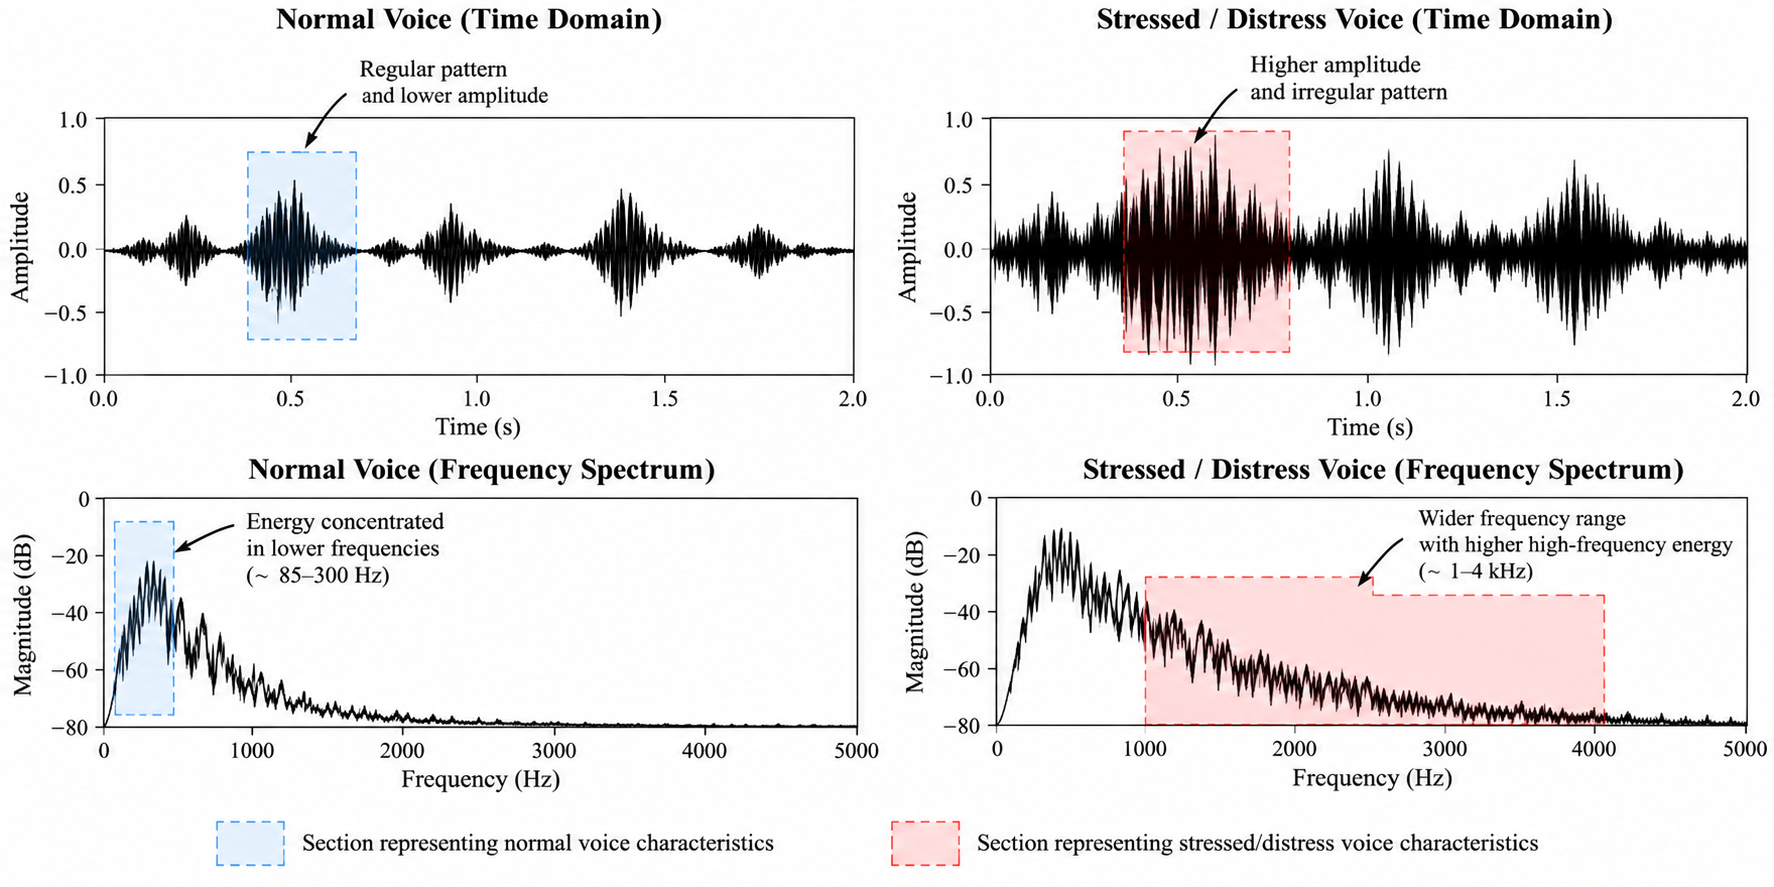
\includegraphics[width=0.85\textwidth]{voice_frequency.png}
\caption{Author-supplied illustrative waveforms and spectra for ordinary and stressed vocalizations. The curves are a conceptual comparison, not recordings from the study or a calibrated rule: amplitude, pitch, and high-frequency energy alone cannot establish distress.}
\label{fig:voice}
\end{figure*}
Fig.~\ref{fig:voice} illustrates why the acoustic task is more than loudness detection. A genuine event can be quiet, distant, or muffled; laughter and excited speech can also be loud and spectrally broad. The model must therefore be tested on both hard negatives and degraded positives before a field dispatch threshold is set.

\subsection{Authenticated Alert and Dispatch}
\label{sec:alert}
The 25-byte packet has a nine-byte clear header (magic, version, node identifier, monotonic counter), an eight-byte encrypted evidence payload, and an eight-byte truncated HMAC tag. The implemented code uses AES-128-CTR and a per-node key derived from a master secret. The hub verifies the tag before decryption and rejects stale counters and unknown nodes. The packet contains no coordinates: the hub resolves the node identifier to surveyed coordinates. The audio clip stays on the local Wi-Fi path, since a four-second PCM clip is much larger than the LoRa alert. Persistent counter handling, key separation, and field link reliability still require deployment validation.

This split makes the alert small enough for low-rate radio while keeping the verification recording off that channel. The gateway forwards packet bytes to the hub without making a dispatch decision. The hub first authenticates the packet, then checks the counter against the last accepted value for that node, and finally looks up the surveyed location. A registry miss, invalid tag, or repeated counter ends processing before a mission request is formed. For field use, counters must survive node resets and the master secret must be kept outside the captured field node; those properties have not been established by the SITL run.

\subsection{Drone Response and Safety Controls}
\label{sec:response}
The dashboard and dispatcher pass a verified incident to the flight API. The response software checks the target geofence, serializes missions in a bounded priority queue, and requires the vehicle to be landed and disarmed before the next flight. Mode changes are retried through MAVLink until the autopilot's reported mode confirms them. The failsafe arbiter evaluates battery, GPS, link, geofence, and progress; LAND takes precedence over RTL. The SITL mission includes takeoff, transit, hover, a simulated first-aid release, and return.

The mission executor moves through connection, GPS readiness, arming, takeoff, transit, hover, delivery, return, and landing states. Each phase checks the arbiter rather than relying on a single pre-flight assessment. A brief invalid GPS report is debounced; a persistent loss requests LAND because a GPS-dependent return is no longer reliable. Battery escalation from low to critical also changes the requested recovery from RTL to LAND. The queue worker checks disarm before beginning another mission, so a second incident cannot start a new takeoff while the first vehicle remains airborne. These are software safeguards layered over the autopilot's own configuration, not evidence of physical flight safety.

\begin{figure}[!t]
\centering
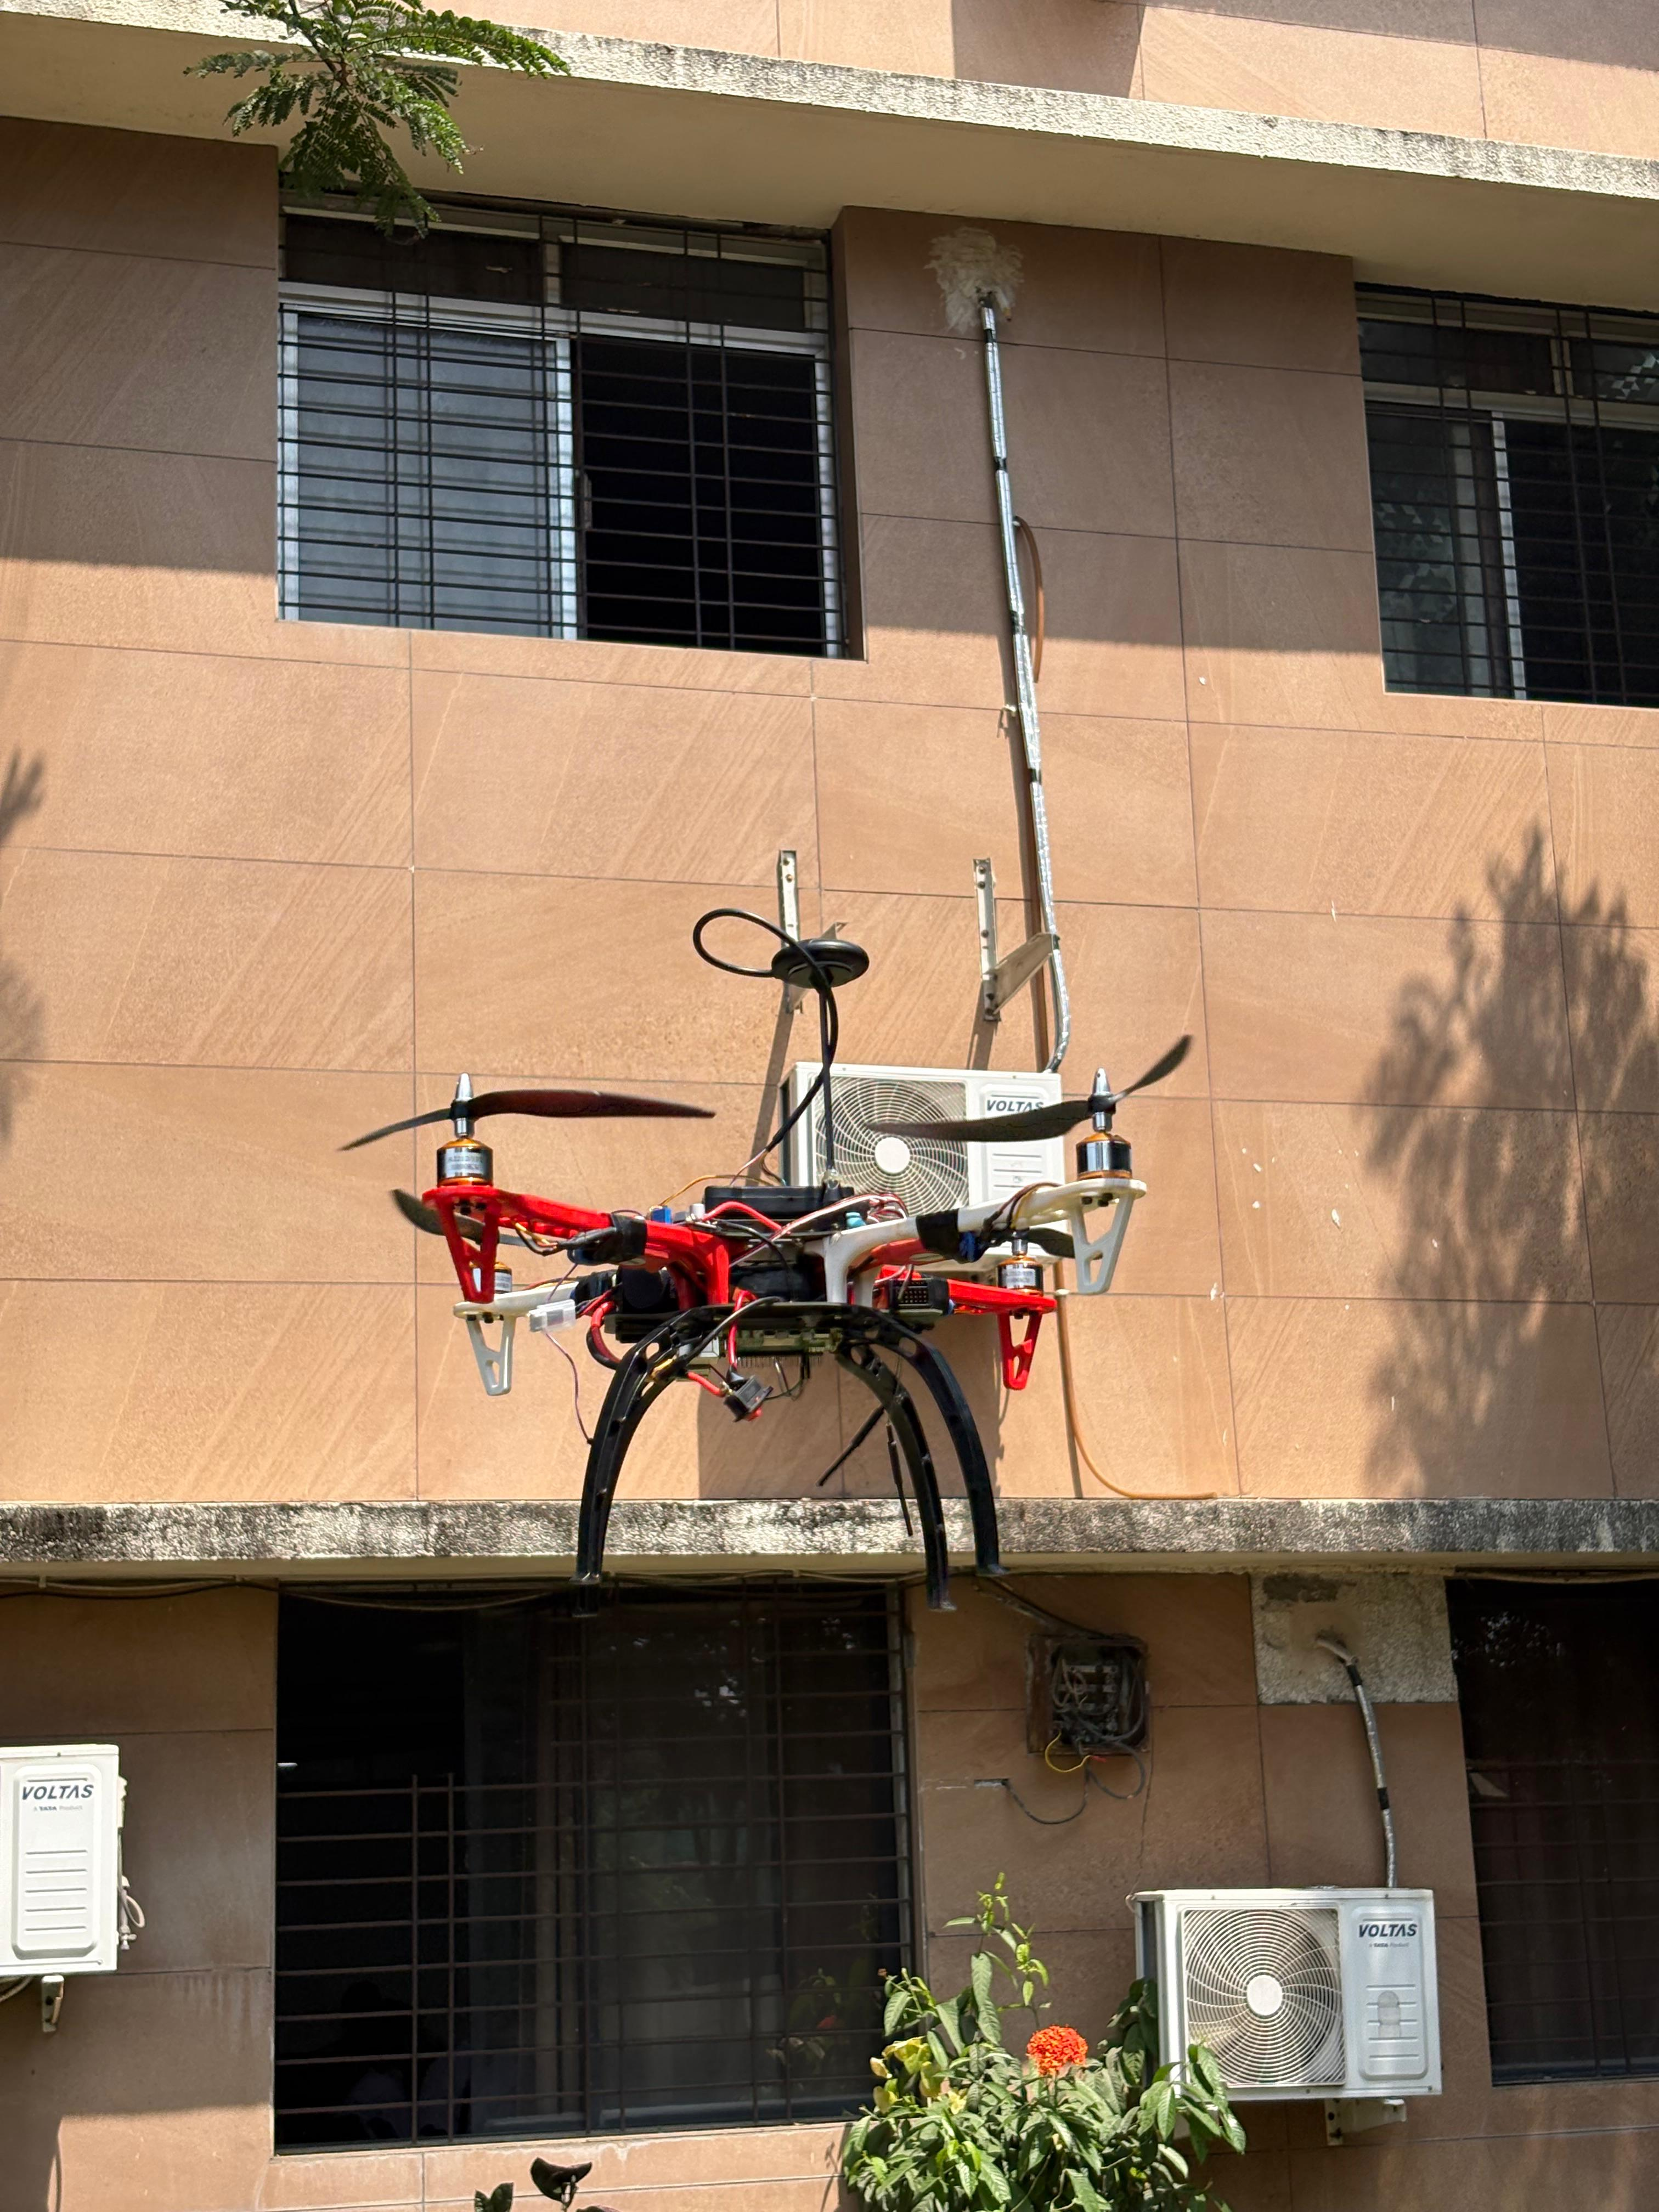
\includegraphics[width=0.78\columnwidth,height=0.24\textheight,keepaspectratio]{drone_supervised_hover.jpeg}
\caption{Author-supplied photograph of the assembled quadcopter during supervised hover. The image documents the airframe, not an end-to-end autonomous flight or a measured payload-delivery result.}
\label{fig:airframe}
\end{figure}
Fig.~\ref{fig:airframe} shows the physical airframe. Current operator-controlled real-mode gates remain disabled pending manual outdoor validation, GPS and battery readiness, and microphone false-alarm testing. The flight photograph should therefore be read separately from the SITL performance reported below.

The proposed delivery sequence descends from observation height, releases the kit only near the ground, then climbs and returns. The release command is recorded as an outcome: a failed actuation must be visible to the operator, but it must not hold the aircraft above the incident indefinitely. The control software can exercise that sequence in simulation; actual drop accuracy, bystander clearance, and camera tracking have not been measured here.

\section{Implementation and Results}
\label{sec:results}

\subsection{Offline Audio and Software Evaluation}
The held-out Stage-1 evaluation used 1,719 clips; Table~\ref{tab:classifier} gives class-wise results. Overall accuracy was 86.62\%, with macro F1 of 0.79 and weighted F1 of 0.86. The scream recall of 0.56 means that 44\% of labelled screams in this split were missed. The 14 help clips are too few to support a broad language or field claim. The reported result applies to the offline model and cannot be used as a false-dispatch rate for the complete system.

\begin{table}[!t]
\caption{Held-Out Stage-1 Acoustic Classifier Results}
\label{tab:classifier}
\centering\footnotesize
\begin{tabular}{|l|c|c|c|c|}
\hline
\textbf{Class} & \textbf{Precision} & \textbf{Recall} & \textbf{F1-score} & \textbf{Support} \\ \hline
Background & 0.92 & 0.93 & 0.92 & 1386 \\ \hline
Scream & 0.66 & 0.56 & 0.60 & 281 \\ \hline
Cry & 0.54 & 0.95 & 0.69 & 38 \\ \hline
Help & 0.88 & 1.00 & 0.93 & 14 \\ \hline
Overall accuracy & \multicolumn{3}{c|}{0.866} & 1719 \\ \hline
Macro F1-score & \multicolumn{3}{c|}{0.79} & 1719 \\ \hline
Weighted F1-score & \multicolumn{3}{c|}{0.86} & 1719 \\ \hline
\end{tabular}
\end{table}

The ArduCopter SITL acceptance run passed eight of eight checks, including arming, target arrival, hover, RTL, and landed/disarmed completion. It reached 0.4 m closest approach against a 5 m arrival tolerance and took 328 s from trigger to disarm. In a separate full-chain rehearsal, a sealed alert passed registry lookup and fusion (severity 0.88), the simulated aircraft descended to about 3.1 m, a servo release was commanded, and the mission ended in COMPLETED. The rehearsal used heuristic acoustic stand-ins. The original 68 unit verifications passed for packet rejection, fusion, queueing, geofence, and flight-safety behaviour; the current repository has added further tests, so 68 is a historical verified count rather than a claim about the current total.

\subsection{Comparative Matrix}
Table~\ref{tab:comparison} preserves the journal comparison. It compares trigger ownership and response workflow; model accuracies across different datasets do not establish a ranking among systems.
\begin{table*}[!t]
\caption{Comparative Matrix: Operational Improvement of VanniKawachh}
\label{tab:comparison}
\centering\scriptsize
\begin{tabular}{|p{3.2cm}|p{3.5cm}|p{2.8cm}|p{3.2cm}|p{4.1cm}|}
\hline
\textbf{System category} & \textbf{Who provides the trigger?} & \textbf{Communication dependence} & \textbf{Response after detection} & \textbf{Operational improvement in VanniKawachh} \\ \hline
Smartphone audio application~\cite{pavithra2026} & Victim and personal phone & Mobile data or phone connectivity & Emergency notification or automation & Fixed nodes can detect a distress call even when a phone is unavailable. \\ \hline
Wearable IoT safety device~\cite{bharathi2025} & Victim and wearable & GPS plus mobile/IoT connection & Alert to contacts or services & No wearable must be charged, carried, or activated by the victim. \\ \hline
Acoustic detection model~\cite{kim2025,fime2024} & Nearby microphone or dataset input & Usually a computing platform; response path not defined & Classification score or alert & Adds contextual verification, encrypted location delivery, and a response workflow. \\ \hline
Manual GPS/GSM tracker~\cite{uganya2023} & Victim presses a button & GSM coverage & Location sharing & Removes the manual action and offers LoRa for low-connectivity locations. \\ \hline
\textbf{VanniKawachh} & \textbf{Infrastructure-mounted acoustic node} & \textbf{Authenticated LoRa alert; no SIM required} & \textbf{Dashboard alert, queued drone mission, evidence capture, payload action, and return} & \textbf{Combines device-independent triggering, two-stage confirmation, security controls, and a safety-checked aerial response.} \\ \hline
\end{tabular}
\end{table*}
\subsection{Evaluation Analysis}
\textbf{Reading the acoustic result.} The test split is dominated by background clips (1,386 of 1,719). This makes overall accuracy a poor stand-alone measure of emergency usefulness: the minority scream class is the one for which a missed event matters most. The model found only 56\% of the 281 labelled screams. Cry recall was higher, but its support was 38 clips; the apparent perfect recall for help comes from just 14 clips. These counts limit the strength of any claim about unfamiliar voices, languages, recording distances, or street noise. The supplied spectrum illustration is helpful for explaining the problem, but no decision threshold or performance estimate was derived from that image.

\textbf{Flight acceptance and failure paths.} The SITL harness launched the flight stack and simulated ArduCopter, sent a request through the same HTTP interface used by the dispatch service, then read vehicle telemetry until landing. The eight checks cover acceptance, connection, arming, altitude, target approach, hover, RTL, and disarmed completion. The 0.4 m figure is the closest simulated approach to the requested coordinate, not a field localization error and not a first-aid drop error. The 328 s wall-clock duration includes the entire simulated mission, so it should not be presented as time to first contact. Unit checks separately exercise a corrupted packet tag, a stale replay counter, sub-threshold fusion, GPS debounce, LAND-over-RTL escalation, and refusal to start a queued mission against an armed vehicle. They test the implemented branches; they cannot establish that a damaged radio, uncalibrated sensor, or windy airframe will behave the same way.

\textbf{Chain rehearsal.} The sealed alert used a registry node and a development audio score to drive the downstream interfaces. The hub accepted the packet, resolved the stored coordinates, computed severity, and sent one mission request. The aircraft then followed the mission sequence in SITL. That rehearsal demonstrates that the modules can exchange the expected data and that the simulated mission can terminate cleanly. It does not evaluate the trained Stage-1 model and hub verifier together on the same live outdoor event. A defensible end-to-end detection rate will require one synchronized test set spanning the microphone, alert link, clip link, hub decision, and response outcome.




\section{Discussion}
\label{sec:discussion}
The present evidence supports a modular prototype and simulated flight chain. Field deployment would need a continuous-background false-alert rate, varied female speech and distress recordings, measured radio range and power, and physical flight tests with an operator. Audio is processed locally until a candidate event, but clips and camera evidence still require access control, retention rules, and notice. Physical UAS operation requires review against current airspace and pilot rules; radio-band use must be checked against the applicable Indian spectrum notification. The prototype's cloud dashboard and phone path do not imply that a LoRa-only field node can reach an internet-hosted service without a local gateway.

The decision policy also has a human consequence. Refusing dispatch without a verification clip protects against a single noisy sensor launching an aircraft, but it cannot help someone whose alert packet arrives while the local clip link fails. A field study should record that failure rate and compare it with a supervised escalation path, such as sending an operator-visible incident without automatic flight. The hub is a locality-level dependency as well: losing it stops authentication, lookup, and dispatch even if pole nodes continue to hear sound. Redundant gateways and a defined recovery procedure belong in a deployment design, not in the performance claims of this prototype.

\section{Conclusion and Future Work}
\label{sec:conclusion}
VanniKawachh connects fixed acoustic sensing, authenticated alerting, contextual verification, and a safety-interlocked drone response. Its offline classifier and SITL results establish separate technical baselines, while the complete field detection-to-flight rate remains unmeasured. The next evaluation should deploy the trained screen on the intended microphone, test hard negatives and muffled calls on unseen speakers, measure the two radio links, and then conduct controlled visual-line-of-sight flights. These measurements will determine whether the combined chain can support supervised emergency use.

\section*{Acknowledgment}
The authors thank the Department of Computer Science and Engineering, G. H. Raisoni College of Engineering, Nagpur, for laboratory access and institutional support.

\balance
\begin{thebibliography}{99}
\bibitem{pavithra2026} R. Pavithra, R. Ahalya, and C. Shuruthika, ``Discreet AI-powered women's safety app with audio recognition and emergency automation,'' in \emph{Proc. 2026 IEEE Int. Students' Conf. Electr., Electron. Comput. Sci. (SCEECS)}, Bhopal, India, 2026, pp. 1--6, doi: 10.1109/SCEECS68810.2026.11430037.
\bibitem{potturi2026} S. Potturi, S. Thota, P. Kandukuru, K. U. Kiran, T. V. N. S. G. Srikar, and H. V. Sai, ``An SOS women safety device: Automatic emergency alerts and geo-location sharing with GSM/GPS integration,'' in \emph{Proc. 2026 Int. Conf. Intell. Comput., Netw. Secur. (IC-ICNS)}, Bhubaneswar, India, 2026, pp. 1--6, doi: 10.1109/IC-ICNS68863.2026.11537940.
\bibitem{bharathi2025} P. S. Bharathi, T. Judgi, D. Pradeep, T. S. Arulananth, A. A. A. Samhan, and J. Giri, ``A novel Internet of Things (IoT) enabled women safety system design with emergency alert mechanism,'' in \emph{Proc. 2025 Int. Conf. Frontier Technol. Solutions (ICFTS)}, 2025, pp. 1--7, doi: 10.1109/ICFTS62006.2025.11031774.
\bibitem{snehith2025} R. Snehith, S. Saranya, and N. R. Reddy, ``A smart device for women safety using IoT,'' in \emph{Proc. 2025 7th Int. Conf. Intell. Sustain. Syst. (ICISS)}, 2025, pp. 277--282, doi: 10.1109/ICISS63372.2025.11076270.
\bibitem{hadkar2024} R. V. Hadkar, A. P. Phadke, H. Satpute, K. Raut, and P. Deshpande, ``An efficient IoT-enabled women safety device,'' in \emph{Proc. 2024 3rd Int. Conf. Autom., Comput. Renew. Syst. (ICACRS)}, 2024, pp. 425--431, doi: 10.1109/ICACRS62842.2024.10841797.
\bibitem{uganya2023} G. Uganya, N. Kirubakaran, T. Bernatin, and M. Boobalan, ``Smart women safety device using IoT and GPS tracker,'' in \emph{Proc. 2023 Intell. Comput. Control Eng. Bus. Syst. (ICCEBS)}, Chennai, India, 2023, pp. 1--6, doi: 10.1109/ICCEBS58601.2023.10449302.
\bibitem{ciaburro2026} G. Ciaburro and V. Puyana-Romero, ``Sound event detection in smart cities: A systematic review of methods, datasets, and applications,'' \emph{Big Data Cogn. Comput.}, vol. 10, no. 3, art. no. 83, 2026, doi: 10.3390/bdcc10030083.
\bibitem{kim2025} Y. Kim, D. Jang, and S.-P. Lee, ``Robust scream detection and scream temporal interval prediction using CNN-Transformer and windowing CNN,'' \emph{IEEE Access}, vol. 13, pp. 71374--71387, 2025, doi: 10.1109/ACCESS.2025.3556729.
\bibitem{kim2024} Y. Kim, D. Jang, and J. Lee, ``Development of scream detection system with large-scale scream dataset,'' in \emph{Proc. 2024 15th Int. Conf. Inf. Commun. Technol. Converg. (ICTC)}, Jeju, South Korea, 2024, pp. 590--593, doi: 10.1109/ICTC62082.2024.10826757.
\bibitem{sharma2025} P. Sharma and T. J. Jebaseeli, ``Smart scream and panic detection system for women using AI,'' in \emph{Proc. 2025 4th Int. Conf. Autom., Comput. Renew. Syst. (ICACRS)}, 2025, pp. 1554--1559, doi: 10.1109/ICACRS67045.2025.11324333.
\bibitem{srimathi2025} A. Srimathi, S. Jothi, and M. P. Sindhiya, ``Human scream detection and analysis for crime reduction,'' in \emph{Proc. 2025 Int. Conf. Multi-Agent Syst. Collaborative Intell. (ICMSCI)}, Erode, India, 2025, pp. 1528--1534, doi: 10.1109/ICMSCI62561.2025.10894058.
\bibitem{fime2024} A. A. Fime, M. Ashikuzzaman, and A. Aziz, ``Audio signal-based danger detection using signal processing and deep learning,'' \emph{Expert Syst. Appl.}, vol. 237, art. no. 121646, Mar. 2024, doi: 10.1016/j.eswa.2023.121646.
\bibitem{trigkas2026} A. Trigkas, D. Piromalis, and P. Papageorgas, ``A federated approach for adaptive urban sound classification on TinyML edge devices,'' \emph{Sensors}, vol. 26, no. 9, art. no. 2854, 2026, doi: 10.3390/s26092854.
\bibitem{david2021} R. David \emph{et al.}, ``TensorFlow Lite Micro: Embedded machine learning for TinyML systems,'' in \emph{Proc. Mach. Learn. Syst. (MLSys)}, vol. 3, 2021, pp. 800--811.
\bibitem{kong2020} Q. Kong, Y. Cao, T. Iqbal, Y. Wang, W. Wang, and M. D. Plumbley, ``PANNs: Large-scale pretrained audio neural networks for audio pattern recognition,'' \emph{IEEE/ACM Trans. Audio, Speech, Lang. Process.}, vol. 28, pp. 2880--2894, 2020, doi: 10.1109/TASLP.2020.3030497.
\bibitem{gemmeke2017} J. F. Gemmeke \emph{et al.}, ``Audio Set: An ontology and human-labeled dataset for audio events,'' in \emph{Proc. IEEE Int. Conf. Acoust., Speech, Signal Process. (ICASSP)}, New Orleans, LA, USA, 2017, pp. 776--780, doi: 10.1109/ICASSP.2017.7952261.
\bibitem{davis1980} S. Davis and P. Mermelstein, ``Comparison of parametric representations for monosyllabic word recognition in continuously spoken sentences,'' \emph{IEEE Trans. Acoust., Speech, Signal Process.}, vol. 28, no. 4, pp. 357--366, Aug. 1980, doi: 10.1109/TASSP.1980.1163420.
\bibitem{sciullo2020} L. Sciullo, A. Trotta, and M. Di Felice, ``Design and performance evaluation of a LoRa-based mobile emergency management system (LOCATE),'' \emph{Ad Hoc Netw.}, vol. 96, art. no. 101993, 2020, doi: 10.1016/j.adhoc.2019.101993.
\bibitem{smith2025} C. M. Smith, C. Powell, C. J. Bernstein, H. Howe, M. Holt, M. O'Sullivan, K. Couper, and N. Rees, ``The use of drone-delivered automated external defibrillators in the emergency response for out-of-hospital cardiac arrest: A simulation study,'' \emph{Resuscitation Plus}, vol. 25, art. no. 101045, 2025, doi: 10.1016/j.resplu.2025.101045.
\bibitem{fips197} National Institute of Standards and Technology, ``Advanced Encryption Standard (AES),'' FIPS PUB 197, Nov. 2001, doi: 10.6028/NIST.FIPS.197.
\bibitem{rfc2104} H. Krawczyk, M. Bellare, and R. Canetti, ``HMAC: Keyed-hashing for message authentication,'' IETF RFC 2104, Feb. 1997, doi: 10.17487/RFC2104.
\bibitem{sx1278} Semtech Corporation, ``SX1276/77/78/79: 137 MHz to 1020 MHz low power long range transceiver,'' datasheet, Rev. 7, 2020. [Online]. Available: \url{https://www.semtech.com/products/wireless-rf/lora-connect/sx1278}
\bibitem{lorawan} LoRa Alliance Technical Committee, ``LoRaWAN L2 1.0.4 specification,'' 2020. [Online]. Available: \url{https://lora-alliance.org/lorawan-specification/}
\bibitem{ardupilot} ArduPilot Development Team, ``ArduPilot documentation,'' and MAVLink Development Team, ``MAVLink developer guide.'' [Online]. Available: \url{https://ardupilot.org/} and \url{https://mavlink.io/}
\bibitem{dpdp2023} Government of India, ``The Digital Personal Data Protection Act, 2023,'' Act No. 22 of 2023, \emph{The Gazette of India}, Aug. 11, 2023.
\bibitem{dronerules2021} Ministry of Civil Aviation, Government of India, ``The Drone Rules, 2021,'' notification G.S.R. 589(E), \emph{The Gazette of India}, Aug. 25, 2021. [Online]. Available: \url{https://digitalsky.dgca.gov.in}
\bibitem{wpc865} Wireless Planning and Coordination Wing, Department of Telecommunications, Government of India, ``Notification delicensing low-power wireless equipment in the 865--867 MHz band.'' [Online]. Available: \url{https://dot.gov.in/spectrum-management}
\end{thebibliography}

\end{document}
